% Created by tikzDevice version 0.12.6 on 2024-03-24 19:09:35
% !TEX encoding = UTF-8 Unicode
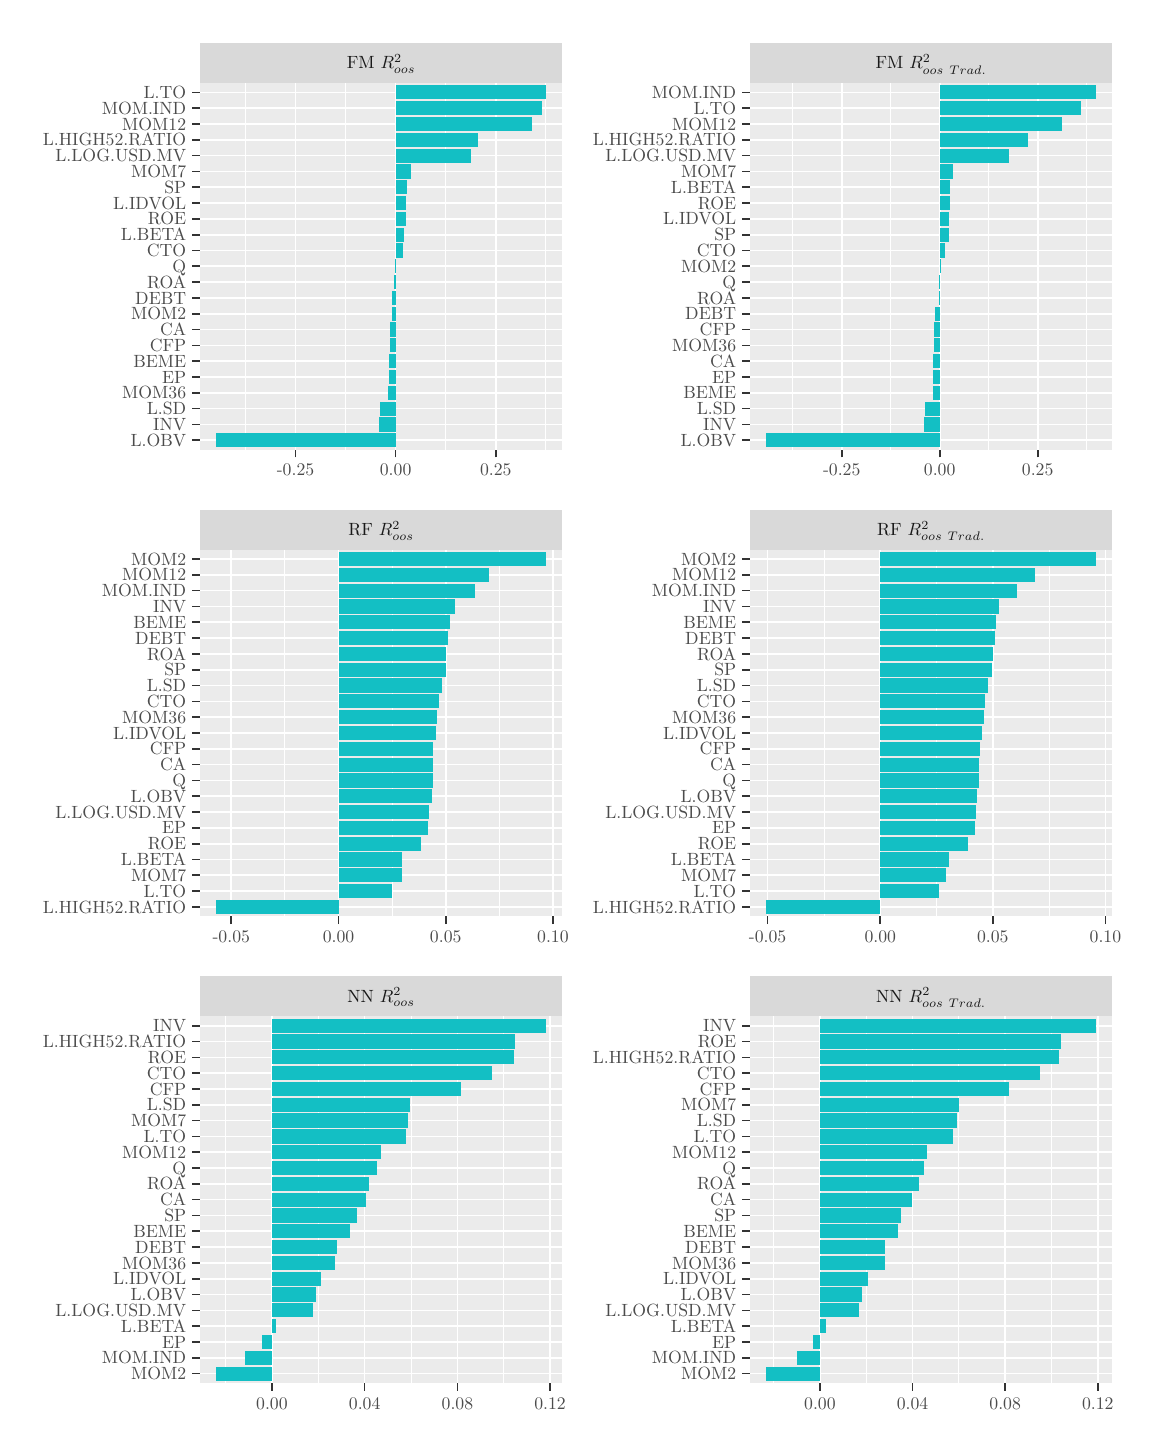
\begin{tikzpicture}[x=1pt,y=1pt]
\definecolor{fillColor}{RGB}{255,255,255}
\path[use as bounding box,fill=fillColor,fill opacity=0.00] (0,0) rectangle (397.48,505.89);
\begin{scope}
\path[clip] (  0.00,337.26) rectangle (198.74,505.89);
\definecolor{drawColor}{RGB}{255,255,255}
\definecolor{fillColor}{RGB}{255,255,255}

\path[draw=drawColor,line width= 0.6pt,line join=round,line cap=round,fill=fillColor] (  0.00,337.26) rectangle (198.74,505.89);
\end{scope}
\begin{scope}
\path[clip] ( 62.22,353.36) rectangle (193.24,485.94);
\definecolor{fillColor}{gray}{0.92}

\path[fill=fillColor] ( 62.22,353.36) rectangle (193.24,485.94);
\definecolor{drawColor}{RGB}{255,255,255}

\path[draw=drawColor,line width= 0.3pt,line join=round] ( 78.70,353.36) --
	( 78.70,485.94);

\path[draw=drawColor,line width= 0.3pt,line join=round] (114.88,353.36) --
	(114.88,485.94);

\path[draw=drawColor,line width= 0.3pt,line join=round] (151.05,353.36) --
	(151.05,485.94);

\path[draw=drawColor,line width= 0.3pt,line join=round] (187.23,353.36) --
	(187.23,485.94);

\path[draw=drawColor,line width= 0.6pt,line join=round] ( 62.22,356.79) --
	(193.24,356.79);

\path[draw=drawColor,line width= 0.6pt,line join=round] ( 62.22,362.51) --
	(193.24,362.51);

\path[draw=drawColor,line width= 0.6pt,line join=round] ( 62.22,368.22) --
	(193.24,368.22);

\path[draw=drawColor,line width= 0.6pt,line join=round] ( 62.22,373.93) --
	(193.24,373.93);

\path[draw=drawColor,line width= 0.6pt,line join=round] ( 62.22,379.65) --
	(193.24,379.65);

\path[draw=drawColor,line width= 0.6pt,line join=round] ( 62.22,385.36) --
	(193.24,385.36);

\path[draw=drawColor,line width= 0.6pt,line join=round] ( 62.22,391.08) --
	(193.24,391.08);

\path[draw=drawColor,line width= 0.6pt,line join=round] ( 62.22,396.79) --
	(193.24,396.79);

\path[draw=drawColor,line width= 0.6pt,line join=round] ( 62.22,402.51) --
	(193.24,402.51);

\path[draw=drawColor,line width= 0.6pt,line join=round] ( 62.22,408.22) --
	(193.24,408.22);

\path[draw=drawColor,line width= 0.6pt,line join=round] ( 62.22,413.94) --
	(193.24,413.94);

\path[draw=drawColor,line width= 0.6pt,line join=round] ( 62.22,419.65) --
	(193.24,419.65);

\path[draw=drawColor,line width= 0.6pt,line join=round] ( 62.22,425.36) --
	(193.24,425.36);

\path[draw=drawColor,line width= 0.6pt,line join=round] ( 62.22,431.08) --
	(193.24,431.08);

\path[draw=drawColor,line width= 0.6pt,line join=round] ( 62.22,436.79) --
	(193.24,436.79);

\path[draw=drawColor,line width= 0.6pt,line join=round] ( 62.22,442.51) --
	(193.24,442.51);

\path[draw=drawColor,line width= 0.6pt,line join=round] ( 62.22,448.22) --
	(193.24,448.22);

\path[draw=drawColor,line width= 0.6pt,line join=round] ( 62.22,453.94) --
	(193.24,453.94);

\path[draw=drawColor,line width= 0.6pt,line join=round] ( 62.22,459.65) --
	(193.24,459.65);

\path[draw=drawColor,line width= 0.6pt,line join=round] ( 62.22,465.37) --
	(193.24,465.37);

\path[draw=drawColor,line width= 0.6pt,line join=round] ( 62.22,471.08) --
	(193.24,471.08);

\path[draw=drawColor,line width= 0.6pt,line join=round] ( 62.22,476.79) --
	(193.24,476.79);

\path[draw=drawColor,line width= 0.6pt,line join=round] ( 62.22,482.51) --
	(193.24,482.51);

\path[draw=drawColor,line width= 0.6pt,line join=round] ( 96.79,353.36) --
	( 96.79,485.94);

\path[draw=drawColor,line width= 0.6pt,line join=round] (132.96,353.36) --
	(132.96,485.94);

\path[draw=drawColor,line width= 0.6pt,line join=round] (169.14,353.36) --
	(169.14,485.94);
\definecolor{fillColor}{RGB}{19,191,196}

\path[fill=fillColor] (130.99,394.22) rectangle (132.96,399.36);

\path[fill=fillColor] (132.96,422.79) rectangle (135.58,427.94);

\path[fill=fillColor] (130.56,382.79) rectangle (132.96,387.93);

\path[fill=fillColor] (130.92,388.51) rectangle (132.96,393.65);

\path[fill=fillColor] (126.96,359.93) rectangle (132.96,365.08);

\path[fill=fillColor] (131.76,405.65) rectangle (132.96,410.79);

\path[fill=fillColor] (132.96,445.65) rectangle (136.90,450.79);

\path[fill=fillColor] (130.49,377.08) rectangle (132.96,382.22);

\path[fill=fillColor] (132.55,411.36) rectangle (132.96,416.51);

\path[fill=fillColor] (132.96,434.22) rectangle (136.57,439.36);

\path[fill=fillColor] (132.90,417.08) rectangle (132.96,422.22);

\path[fill=fillColor] (132.96,451.37) rectangle (138.34,456.51);

\path[fill=fillColor] (132.96,468.51) rectangle (182.41,473.65);

\path[fill=fillColor] (130.38,371.36) rectangle (132.96,376.51);

\path[fill=fillColor] (131.63,399.94) rectangle (132.96,405.08);

\path[fill=fillColor] (132.96,474.22) rectangle (185.98,479.37);

\path[fill=fillColor] (127.27,365.65) rectangle (132.96,370.79);

\path[fill=fillColor] (132.96,462.79) rectangle (162.64,467.94);

\path[fill=fillColor] (132.96,428.51) rectangle (135.89,433.65);

\path[fill=fillColor] (132.96,439.94) rectangle (136.60,445.08);

\path[fill=fillColor] (132.96,457.08) rectangle (160.11,462.22);

\path[fill=fillColor] (132.96,479.94) rectangle (187.29,485.08);

\path[fill=fillColor] ( 68.17,354.22) rectangle (132.96,359.36);
\end{scope}
\begin{scope}
\path[clip] ( 62.22,485.94) rectangle (193.24,500.39);
\definecolor{fillColor}{gray}{0.85}

\path[fill=fillColor] ( 62.22,485.94) rectangle (193.24,500.39);
\definecolor{drawColor}{gray}{0.10}

\node[text=drawColor,anchor=base,inner sep=0pt, outer sep=0pt, scale=  0.64] at (127.73,490.96) {FM $R^2_{oos}$};
\end{scope}
\begin{scope}
\path[clip] (  0.00,  0.00) rectangle (397.48,505.89);
\definecolor{drawColor}{gray}{0.20}

\path[draw=drawColor,line width= 0.6pt,line join=round] ( 96.79,350.61) --
	( 96.79,353.36);

\path[draw=drawColor,line width= 0.6pt,line join=round] (132.96,350.61) --
	(132.96,353.36);

\path[draw=drawColor,line width= 0.6pt,line join=round] (169.14,350.61) --
	(169.14,353.36);
\end{scope}
\begin{scope}
\path[clip] (  0.00,  0.00) rectangle (397.48,505.89);
\definecolor{drawColor}{gray}{0.30}

\node[text=drawColor,anchor=base,inner sep=0pt, outer sep=0pt, scale=  0.64] at ( 96.79,344.00) {-0.25};

\node[text=drawColor,anchor=base,inner sep=0pt, outer sep=0pt, scale=  0.64] at (132.96,344.00) {0.00};

\node[text=drawColor,anchor=base,inner sep=0pt, outer sep=0pt, scale=  0.64] at (169.14,344.00) {0.25};
\end{scope}
\begin{scope}
\path[clip] (  0.00,  0.00) rectangle (397.48,505.89);
\definecolor{drawColor}{gray}{0.30}

\node[text=drawColor,anchor=base east,inner sep=0pt, outer sep=0pt, scale=  0.64] at ( 57.27,354.59) {L.OBV};

\node[text=drawColor,anchor=base east,inner sep=0pt, outer sep=0pt, scale=  0.64] at ( 57.27,360.30) {INV};

\node[text=drawColor,anchor=base east,inner sep=0pt, outer sep=0pt, scale=  0.64] at ( 57.27,366.02) {L.SD};

\node[text=drawColor,anchor=base east,inner sep=0pt, outer sep=0pt, scale=  0.64] at ( 57.27,371.73) {MOM36};

\node[text=drawColor,anchor=base east,inner sep=0pt, outer sep=0pt, scale=  0.64] at ( 57.27,377.44) {EP};

\node[text=drawColor,anchor=base east,inner sep=0pt, outer sep=0pt, scale=  0.64] at ( 57.27,383.16) {BEME};

\node[text=drawColor,anchor=base east,inner sep=0pt, outer sep=0pt, scale=  0.64] at ( 57.27,388.87) {CFP};

\node[text=drawColor,anchor=base east,inner sep=0pt, outer sep=0pt, scale=  0.64] at ( 57.27,394.59) {CA};

\node[text=drawColor,anchor=base east,inner sep=0pt, outer sep=0pt, scale=  0.64] at ( 57.27,400.30) {MOM2};

\node[text=drawColor,anchor=base east,inner sep=0pt, outer sep=0pt, scale=  0.64] at ( 57.27,406.02) {DEBT};

\node[text=drawColor,anchor=base east,inner sep=0pt, outer sep=0pt, scale=  0.64] at ( 57.27,411.73) {ROA};

\node[text=drawColor,anchor=base east,inner sep=0pt, outer sep=0pt, scale=  0.64] at ( 57.27,417.45) {Q};

\node[text=drawColor,anchor=base east,inner sep=0pt, outer sep=0pt, scale=  0.64] at ( 57.27,423.16) {CTO};

\node[text=drawColor,anchor=base east,inner sep=0pt, outer sep=0pt, scale=  0.64] at ( 57.27,428.88) {L.BETA};

\node[text=drawColor,anchor=base east,inner sep=0pt, outer sep=0pt, scale=  0.64] at ( 57.27,434.59) {ROE};

\node[text=drawColor,anchor=base east,inner sep=0pt, outer sep=0pt, scale=  0.64] at ( 57.27,440.30) {L.IDVOL};

\node[text=drawColor,anchor=base east,inner sep=0pt, outer sep=0pt, scale=  0.64] at ( 57.27,446.02) {SP};

\node[text=drawColor,anchor=base east,inner sep=0pt, outer sep=0pt, scale=  0.64] at ( 57.27,451.73) {MOM7};

\node[text=drawColor,anchor=base east,inner sep=0pt, outer sep=0pt, scale=  0.64] at ( 57.27,457.45) {L.LOG.USD.MV};

\node[text=drawColor,anchor=base east,inner sep=0pt, outer sep=0pt, scale=  0.64] at ( 57.27,463.16) {L.HIGH52.RATIO};

\node[text=drawColor,anchor=base east,inner sep=0pt, outer sep=0pt, scale=  0.64] at ( 57.27,468.88) {MOM12};

\node[text=drawColor,anchor=base east,inner sep=0pt, outer sep=0pt, scale=  0.64] at ( 57.27,474.59) {MOM.IND};

\node[text=drawColor,anchor=base east,inner sep=0pt, outer sep=0pt, scale=  0.64] at ( 57.27,480.31) {L.TO};
\end{scope}
\begin{scope}
\path[clip] (  0.00,  0.00) rectangle (397.48,505.89);
\definecolor{drawColor}{gray}{0.20}

\path[draw=drawColor,line width= 0.6pt,line join=round] ( 59.47,356.79) --
	( 62.22,356.79);

\path[draw=drawColor,line width= 0.6pt,line join=round] ( 59.47,362.51) --
	( 62.22,362.51);

\path[draw=drawColor,line width= 0.6pt,line join=round] ( 59.47,368.22) --
	( 62.22,368.22);

\path[draw=drawColor,line width= 0.6pt,line join=round] ( 59.47,373.93) --
	( 62.22,373.93);

\path[draw=drawColor,line width= 0.6pt,line join=round] ( 59.47,379.65) --
	( 62.22,379.65);

\path[draw=drawColor,line width= 0.6pt,line join=round] ( 59.47,385.36) --
	( 62.22,385.36);

\path[draw=drawColor,line width= 0.6pt,line join=round] ( 59.47,391.08) --
	( 62.22,391.08);

\path[draw=drawColor,line width= 0.6pt,line join=round] ( 59.47,396.79) --
	( 62.22,396.79);

\path[draw=drawColor,line width= 0.6pt,line join=round] ( 59.47,402.51) --
	( 62.22,402.51);

\path[draw=drawColor,line width= 0.6pt,line join=round] ( 59.47,408.22) --
	( 62.22,408.22);

\path[draw=drawColor,line width= 0.6pt,line join=round] ( 59.47,413.94) --
	( 62.22,413.94);

\path[draw=drawColor,line width= 0.6pt,line join=round] ( 59.47,419.65) --
	( 62.22,419.65);

\path[draw=drawColor,line width= 0.6pt,line join=round] ( 59.47,425.36) --
	( 62.22,425.36);

\path[draw=drawColor,line width= 0.6pt,line join=round] ( 59.47,431.08) --
	( 62.22,431.08);

\path[draw=drawColor,line width= 0.6pt,line join=round] ( 59.47,436.79) --
	( 62.22,436.79);

\path[draw=drawColor,line width= 0.6pt,line join=round] ( 59.47,442.51) --
	( 62.22,442.51);

\path[draw=drawColor,line width= 0.6pt,line join=round] ( 59.47,448.22) --
	( 62.22,448.22);

\path[draw=drawColor,line width= 0.6pt,line join=round] ( 59.47,453.94) --
	( 62.22,453.94);

\path[draw=drawColor,line width= 0.6pt,line join=round] ( 59.47,459.65) --
	( 62.22,459.65);

\path[draw=drawColor,line width= 0.6pt,line join=round] ( 59.47,465.37) --
	( 62.22,465.37);

\path[draw=drawColor,line width= 0.6pt,line join=round] ( 59.47,471.08) --
	( 62.22,471.08);

\path[draw=drawColor,line width= 0.6pt,line join=round] ( 59.47,476.79) --
	( 62.22,476.79);

\path[draw=drawColor,line width= 0.6pt,line join=round] ( 59.47,482.51) --
	( 62.22,482.51);
\end{scope}
\begin{scope}
\path[clip] (198.74,337.26) rectangle (397.48,505.89);
\definecolor{drawColor}{RGB}{255,255,255}
\definecolor{fillColor}{RGB}{255,255,255}

\path[draw=drawColor,line width= 0.6pt,line join=round,line cap=round,fill=fillColor] (198.74,337.26) rectangle (397.48,505.89);
\end{scope}
\begin{scope}
\path[clip] (260.96,353.36) rectangle (391.98,485.94);
\definecolor{fillColor}{gray}{0.92}

\path[fill=fillColor] (260.96,353.36) rectangle (391.98,485.94);
\definecolor{drawColor}{RGB}{255,255,255}

\path[draw=drawColor,line width= 0.3pt,line join=round] (276.46,353.36) --
	(276.46,485.94);

\path[draw=drawColor,line width= 0.3pt,line join=round] (311.86,353.36) --
	(311.86,485.94);

\path[draw=drawColor,line width= 0.3pt,line join=round] (347.26,353.36) --
	(347.26,485.94);

\path[draw=drawColor,line width= 0.3pt,line join=round] (382.66,353.36) --
	(382.66,485.94);

\path[draw=drawColor,line width= 0.6pt,line join=round] (260.96,356.79) --
	(391.98,356.79);

\path[draw=drawColor,line width= 0.6pt,line join=round] (260.96,362.51) --
	(391.98,362.51);

\path[draw=drawColor,line width= 0.6pt,line join=round] (260.96,368.22) --
	(391.98,368.22);

\path[draw=drawColor,line width= 0.6pt,line join=round] (260.96,373.93) --
	(391.98,373.93);

\path[draw=drawColor,line width= 0.6pt,line join=round] (260.96,379.65) --
	(391.98,379.65);

\path[draw=drawColor,line width= 0.6pt,line join=round] (260.96,385.36) --
	(391.98,385.36);

\path[draw=drawColor,line width= 0.6pt,line join=round] (260.96,391.08) --
	(391.98,391.08);

\path[draw=drawColor,line width= 0.6pt,line join=round] (260.96,396.79) --
	(391.98,396.79);

\path[draw=drawColor,line width= 0.6pt,line join=round] (260.96,402.51) --
	(391.98,402.51);

\path[draw=drawColor,line width= 0.6pt,line join=round] (260.96,408.22) --
	(391.98,408.22);

\path[draw=drawColor,line width= 0.6pt,line join=round] (260.96,413.94) --
	(391.98,413.94);

\path[draw=drawColor,line width= 0.6pt,line join=round] (260.96,419.65) --
	(391.98,419.65);

\path[draw=drawColor,line width= 0.6pt,line join=round] (260.96,425.36) --
	(391.98,425.36);

\path[draw=drawColor,line width= 0.6pt,line join=round] (260.96,431.08) --
	(391.98,431.08);

\path[draw=drawColor,line width= 0.6pt,line join=round] (260.96,436.79) --
	(391.98,436.79);

\path[draw=drawColor,line width= 0.6pt,line join=round] (260.96,442.51) --
	(391.98,442.51);

\path[draw=drawColor,line width= 0.6pt,line join=round] (260.96,448.22) --
	(391.98,448.22);

\path[draw=drawColor,line width= 0.6pt,line join=round] (260.96,453.94) --
	(391.98,453.94);

\path[draw=drawColor,line width= 0.6pt,line join=round] (260.96,459.65) --
	(391.98,459.65);

\path[draw=drawColor,line width= 0.6pt,line join=round] (260.96,465.37) --
	(391.98,465.37);

\path[draw=drawColor,line width= 0.6pt,line join=round] (260.96,471.08) --
	(391.98,471.08);

\path[draw=drawColor,line width= 0.6pt,line join=round] (260.96,476.79) --
	(391.98,476.79);

\path[draw=drawColor,line width= 0.6pt,line join=round] (260.96,482.51) --
	(391.98,482.51);

\path[draw=drawColor,line width= 0.6pt,line join=round] (294.16,353.36) --
	(294.16,485.94);

\path[draw=drawColor,line width= 0.6pt,line join=round] (329.56,353.36) --
	(329.56,485.94);

\path[draw=drawColor,line width= 0.6pt,line join=round] (364.96,353.36) --
	(364.96,485.94);
\definecolor{fillColor}{RGB}{19,191,196}

\path[fill=fillColor] (327.28,382.79) rectangle (329.56,387.93);

\path[fill=fillColor] (329.56,422.79) rectangle (331.30,427.94);

\path[fill=fillColor] (326.97,371.36) rectangle (329.56,376.51);

\path[fill=fillColor] (327.50,394.22) rectangle (329.56,399.36);

\path[fill=fillColor] (323.82,359.93) rectangle (329.56,365.08);

\path[fill=fillColor] (328.01,399.94) rectangle (329.56,405.08);

\path[fill=fillColor] (329.56,428.51) rectangle (332.74,433.65);

\path[fill=fillColor] (327.02,377.08) rectangle (329.56,382.22);

\path[fill=fillColor] (329.26,405.65) rectangle (329.56,410.79);

\path[fill=fillColor] (329.56,439.94) rectangle (333.14,445.08);

\path[fill=fillColor] (329.45,411.36) rectangle (329.56,416.51);

\path[fill=fillColor] (329.56,451.37) rectangle (334.30,456.51);

\path[fill=fillColor] (329.56,468.51) rectangle (373.74,473.65);

\path[fill=fillColor] (327.45,388.51) rectangle (329.56,393.65);

\path[fill=fillColor] (329.56,417.08) rectangle (329.67,422.22);

\path[fill=fillColor] (329.56,479.94) rectangle (386.03,485.08);

\path[fill=fillColor] (324.37,365.65) rectangle (329.56,370.79);

\path[fill=fillColor] (329.56,462.79) rectangle (361.64,467.94);

\path[fill=fillColor] (329.56,445.65) rectangle (333.22,450.79);

\path[fill=fillColor] (329.56,434.22) rectangle (332.74,439.36);

\path[fill=fillColor] (329.56,457.08) rectangle (354.48,462.22);

\path[fill=fillColor] (329.56,474.22) rectangle (380.48,479.37);

\path[fill=fillColor] (266.91,354.22) rectangle (329.56,359.36);
\end{scope}
\begin{scope}
\path[clip] (260.96,485.94) rectangle (391.98,500.39);
\definecolor{fillColor}{gray}{0.85}

\path[fill=fillColor] (260.96,485.94) rectangle (391.98,500.39);
\definecolor{drawColor}{gray}{0.10}

\node[text=drawColor,anchor=base,inner sep=0pt, outer sep=0pt, scale=  0.64] at (326.47,490.96) {FM $R^2_{oos \ Trad.}$};
\end{scope}
\begin{scope}
\path[clip] (  0.00,  0.00) rectangle (397.48,505.89);
\definecolor{drawColor}{gray}{0.20}

\path[draw=drawColor,line width= 0.6pt,line join=round] (294.16,350.61) --
	(294.16,353.36);

\path[draw=drawColor,line width= 0.6pt,line join=round] (329.56,350.61) --
	(329.56,353.36);

\path[draw=drawColor,line width= 0.6pt,line join=round] (364.96,350.61) --
	(364.96,353.36);
\end{scope}
\begin{scope}
\path[clip] (  0.00,  0.00) rectangle (397.48,505.89);
\definecolor{drawColor}{gray}{0.30}

\node[text=drawColor,anchor=base,inner sep=0pt, outer sep=0pt, scale=  0.64] at (294.16,344.00) {-0.25};

\node[text=drawColor,anchor=base,inner sep=0pt, outer sep=0pt, scale=  0.64] at (329.56,344.00) {0.00};

\node[text=drawColor,anchor=base,inner sep=0pt, outer sep=0pt, scale=  0.64] at (364.96,344.00) {0.25};
\end{scope}
\begin{scope}
\path[clip] (  0.00,  0.00) rectangle (397.48,505.89);
\definecolor{drawColor}{gray}{0.30}

\node[text=drawColor,anchor=base east,inner sep=0pt, outer sep=0pt, scale=  0.64] at (256.01,354.59) {L.OBV};

\node[text=drawColor,anchor=base east,inner sep=0pt, outer sep=0pt, scale=  0.64] at (256.01,360.30) {INV};

\node[text=drawColor,anchor=base east,inner sep=0pt, outer sep=0pt, scale=  0.64] at (256.01,366.02) {L.SD};

\node[text=drawColor,anchor=base east,inner sep=0pt, outer sep=0pt, scale=  0.64] at (256.01,371.73) {BEME};

\node[text=drawColor,anchor=base east,inner sep=0pt, outer sep=0pt, scale=  0.64] at (256.01,377.44) {EP};

\node[text=drawColor,anchor=base east,inner sep=0pt, outer sep=0pt, scale=  0.64] at (256.01,383.16) {CA};

\node[text=drawColor,anchor=base east,inner sep=0pt, outer sep=0pt, scale=  0.64] at (256.01,388.87) {MOM36};

\node[text=drawColor,anchor=base east,inner sep=0pt, outer sep=0pt, scale=  0.64] at (256.01,394.59) {CFP};

\node[text=drawColor,anchor=base east,inner sep=0pt, outer sep=0pt, scale=  0.64] at (256.01,400.30) {DEBT};

\node[text=drawColor,anchor=base east,inner sep=0pt, outer sep=0pt, scale=  0.64] at (256.01,406.02) {ROA};

\node[text=drawColor,anchor=base east,inner sep=0pt, outer sep=0pt, scale=  0.64] at (256.01,411.73) {Q};

\node[text=drawColor,anchor=base east,inner sep=0pt, outer sep=0pt, scale=  0.64] at (256.01,417.45) {MOM2};

\node[text=drawColor,anchor=base east,inner sep=0pt, outer sep=0pt, scale=  0.64] at (256.01,423.16) {CTO};

\node[text=drawColor,anchor=base east,inner sep=0pt, outer sep=0pt, scale=  0.64] at (256.01,428.88) {SP};

\node[text=drawColor,anchor=base east,inner sep=0pt, outer sep=0pt, scale=  0.64] at (256.01,434.59) {L.IDVOL};

\node[text=drawColor,anchor=base east,inner sep=0pt, outer sep=0pt, scale=  0.64] at (256.01,440.30) {ROE};

\node[text=drawColor,anchor=base east,inner sep=0pt, outer sep=0pt, scale=  0.64] at (256.01,446.02) {L.BETA};

\node[text=drawColor,anchor=base east,inner sep=0pt, outer sep=0pt, scale=  0.64] at (256.01,451.73) {MOM7};

\node[text=drawColor,anchor=base east,inner sep=0pt, outer sep=0pt, scale=  0.64] at (256.01,457.45) {L.LOG.USD.MV};

\node[text=drawColor,anchor=base east,inner sep=0pt, outer sep=0pt, scale=  0.64] at (256.01,463.16) {L.HIGH52.RATIO};

\node[text=drawColor,anchor=base east,inner sep=0pt, outer sep=0pt, scale=  0.64] at (256.01,468.88) {MOM12};

\node[text=drawColor,anchor=base east,inner sep=0pt, outer sep=0pt, scale=  0.64] at (256.01,474.59) {L.TO};

\node[text=drawColor,anchor=base east,inner sep=0pt, outer sep=0pt, scale=  0.64] at (256.01,480.31) {MOM.IND};
\end{scope}
\begin{scope}
\path[clip] (  0.00,  0.00) rectangle (397.48,505.89);
\definecolor{drawColor}{gray}{0.20}

\path[draw=drawColor,line width= 0.6pt,line join=round] (258.21,356.79) --
	(260.96,356.79);

\path[draw=drawColor,line width= 0.6pt,line join=round] (258.21,362.51) --
	(260.96,362.51);

\path[draw=drawColor,line width= 0.6pt,line join=round] (258.21,368.22) --
	(260.96,368.22);

\path[draw=drawColor,line width= 0.6pt,line join=round] (258.21,373.93) --
	(260.96,373.93);

\path[draw=drawColor,line width= 0.6pt,line join=round] (258.21,379.65) --
	(260.96,379.65);

\path[draw=drawColor,line width= 0.6pt,line join=round] (258.21,385.36) --
	(260.96,385.36);

\path[draw=drawColor,line width= 0.6pt,line join=round] (258.21,391.08) --
	(260.96,391.08);

\path[draw=drawColor,line width= 0.6pt,line join=round] (258.21,396.79) --
	(260.96,396.79);

\path[draw=drawColor,line width= 0.6pt,line join=round] (258.21,402.51) --
	(260.96,402.51);

\path[draw=drawColor,line width= 0.6pt,line join=round] (258.21,408.22) --
	(260.96,408.22);

\path[draw=drawColor,line width= 0.6pt,line join=round] (258.21,413.94) --
	(260.96,413.94);

\path[draw=drawColor,line width= 0.6pt,line join=round] (258.21,419.65) --
	(260.96,419.65);

\path[draw=drawColor,line width= 0.6pt,line join=round] (258.21,425.36) --
	(260.96,425.36);

\path[draw=drawColor,line width= 0.6pt,line join=round] (258.21,431.08) --
	(260.96,431.08);

\path[draw=drawColor,line width= 0.6pt,line join=round] (258.21,436.79) --
	(260.96,436.79);

\path[draw=drawColor,line width= 0.6pt,line join=round] (258.21,442.51) --
	(260.96,442.51);

\path[draw=drawColor,line width= 0.6pt,line join=round] (258.21,448.22) --
	(260.96,448.22);

\path[draw=drawColor,line width= 0.6pt,line join=round] (258.21,453.94) --
	(260.96,453.94);

\path[draw=drawColor,line width= 0.6pt,line join=round] (258.21,459.65) --
	(260.96,459.65);

\path[draw=drawColor,line width= 0.6pt,line join=round] (258.21,465.37) --
	(260.96,465.37);

\path[draw=drawColor,line width= 0.6pt,line join=round] (258.21,471.08) --
	(260.96,471.08);

\path[draw=drawColor,line width= 0.6pt,line join=round] (258.21,476.79) --
	(260.96,476.79);

\path[draw=drawColor,line width= 0.6pt,line join=round] (258.21,482.51) --
	(260.96,482.51);
\end{scope}
\begin{scope}
\path[clip] (  0.00,168.63) rectangle (198.74,337.26);
\definecolor{drawColor}{RGB}{255,255,255}
\definecolor{fillColor}{RGB}{255,255,255}

\path[draw=drawColor,line width= 0.6pt,line join=round,line cap=round,fill=fillColor] (  0.00,168.63) rectangle (198.74,337.26);
\end{scope}
\begin{scope}
\path[clip] ( 62.22,184.73) rectangle (193.24,317.31);
\definecolor{fillColor}{gray}{0.92}

\path[fill=fillColor] ( 62.22,184.73) rectangle (193.24,317.31);
\definecolor{drawColor}{RGB}{255,255,255}

\path[draw=drawColor,line width= 0.3pt,line join=round] ( 92.94,184.73) --
	( 92.94,317.31);

\path[draw=drawColor,line width= 0.3pt,line join=round] (131.69,184.73) --
	(131.69,317.31);

\path[draw=drawColor,line width= 0.3pt,line join=round] (170.43,184.73) --
	(170.43,317.31);

\path[draw=drawColor,line width= 0.6pt,line join=round] ( 62.22,188.16) --
	(193.24,188.16);

\path[draw=drawColor,line width= 0.6pt,line join=round] ( 62.22,193.88) --
	(193.24,193.88);

\path[draw=drawColor,line width= 0.6pt,line join=round] ( 62.22,199.59) --
	(193.24,199.59);

\path[draw=drawColor,line width= 0.6pt,line join=round] ( 62.22,205.30) --
	(193.24,205.30);

\path[draw=drawColor,line width= 0.6pt,line join=round] ( 62.22,211.02) --
	(193.24,211.02);

\path[draw=drawColor,line width= 0.6pt,line join=round] ( 62.22,216.73) --
	(193.24,216.73);

\path[draw=drawColor,line width= 0.6pt,line join=round] ( 62.22,222.45) --
	(193.24,222.45);

\path[draw=drawColor,line width= 0.6pt,line join=round] ( 62.22,228.16) --
	(193.24,228.16);

\path[draw=drawColor,line width= 0.6pt,line join=round] ( 62.22,233.88) --
	(193.24,233.88);

\path[draw=drawColor,line width= 0.6pt,line join=round] ( 62.22,239.59) --
	(193.24,239.59);

\path[draw=drawColor,line width= 0.6pt,line join=round] ( 62.22,245.31) --
	(193.24,245.31);

\path[draw=drawColor,line width= 0.6pt,line join=round] ( 62.22,251.02) --
	(193.24,251.02);

\path[draw=drawColor,line width= 0.6pt,line join=round] ( 62.22,256.73) --
	(193.24,256.73);

\path[draw=drawColor,line width= 0.6pt,line join=round] ( 62.22,262.45) --
	(193.24,262.45);

\path[draw=drawColor,line width= 0.6pt,line join=round] ( 62.22,268.16) --
	(193.24,268.16);

\path[draw=drawColor,line width= 0.6pt,line join=round] ( 62.22,273.88) --
	(193.24,273.88);

\path[draw=drawColor,line width= 0.6pt,line join=round] ( 62.22,279.59) --
	(193.24,279.59);

\path[draw=drawColor,line width= 0.6pt,line join=round] ( 62.22,285.31) --
	(193.24,285.31);

\path[draw=drawColor,line width= 0.6pt,line join=round] ( 62.22,291.02) --
	(193.24,291.02);

\path[draw=drawColor,line width= 0.6pt,line join=round] ( 62.22,296.74) --
	(193.24,296.74);

\path[draw=drawColor,line width= 0.6pt,line join=round] ( 62.22,302.45) --
	(193.24,302.45);

\path[draw=drawColor,line width= 0.6pt,line join=round] ( 62.22,308.16) --
	(193.24,308.16);

\path[draw=drawColor,line width= 0.6pt,line join=round] ( 62.22,313.88) --
	(193.24,313.88);

\path[draw=drawColor,line width= 0.6pt,line join=round] ( 73.57,184.73) --
	( 73.57,317.31);

\path[draw=drawColor,line width= 0.6pt,line join=round] (112.32,184.73) --
	(112.32,317.31);

\path[draw=drawColor,line width= 0.6pt,line join=round] (151.06,184.73) --
	(151.06,317.31);

\path[draw=drawColor,line width= 0.6pt,line join=round] (189.80,184.73) --
	(189.80,317.31);
\definecolor{fillColor}{RGB}{19,191,196}

\path[fill=fillColor] (112.32,237.02) rectangle (146.46,242.16);

\path[fill=fillColor] (112.32,259.88) rectangle (148.61,265.02);

\path[fill=fillColor] (112.32,288.45) rectangle (152.56,293.59);

\path[fill=fillColor] (112.32,242.73) rectangle (146.60,247.88);

\path[fill=fillColor] (112.32,294.16) rectangle (154.34,299.31);

\path[fill=fillColor] (112.32,282.74) rectangle (151.74,287.88);

\path[fill=fillColor] (112.32,271.31) rectangle (150.98,276.45);

\path[fill=fillColor] (112.32,214.16) rectangle (144.56,219.30);

\path[fill=fillColor] (112.32,277.02) rectangle (151.26,282.16);

\path[fill=fillColor] (112.32,208.45) rectangle (142.07,213.59);

\path[fill=fillColor] (112.32,231.31) rectangle (146.43,236.45);

\path[fill=fillColor] (112.32,197.02) rectangle (135.23,202.16);

\path[fill=fillColor] (112.32,305.59) rectangle (166.77,310.74);

\path[fill=fillColor] (112.32,254.16) rectangle (147.96,259.31);

\path[fill=fillColor] (112.32,311.31) rectangle (187.29,316.45);

\path[fill=fillColor] (112.32,299.88) rectangle (161.81,305.02);

\path[fill=fillColor] (112.32,265.59) rectangle (149.65,270.73);

\path[fill=fillColor] ( 68.17,185.59) rectangle (112.32,190.73);

\path[fill=fillColor] (112.32,202.73) rectangle (135.32,207.88);

\path[fill=fillColor] (112.32,248.45) rectangle (147.66,253.59);

\path[fill=fillColor] (112.32,219.88) rectangle (144.90,225.02);

\path[fill=fillColor] (112.32,191.30) rectangle (131.70,196.45);

\path[fill=fillColor] (112.32,225.59) rectangle (145.98,230.73);
\end{scope}
\begin{scope}
\path[clip] ( 62.22,317.31) rectangle (193.24,331.76);
\definecolor{fillColor}{gray}{0.85}

\path[fill=fillColor] ( 62.22,317.31) rectangle (193.24,331.76);
\definecolor{drawColor}{gray}{0.10}

\node[text=drawColor,anchor=base,inner sep=0pt, outer sep=0pt, scale=  0.64] at (127.73,322.33) {RF $R^2_{oos}$};
\end{scope}
\begin{scope}
\path[clip] (  0.00,  0.00) rectangle (397.48,505.89);
\definecolor{drawColor}{gray}{0.20}

\path[draw=drawColor,line width= 0.6pt,line join=round] ( 73.57,181.98) --
	( 73.57,184.73);

\path[draw=drawColor,line width= 0.6pt,line join=round] (112.32,181.98) --
	(112.32,184.73);

\path[draw=drawColor,line width= 0.6pt,line join=round] (151.06,181.98) --
	(151.06,184.73);

\path[draw=drawColor,line width= 0.6pt,line join=round] (189.80,181.98) --
	(189.80,184.73);
\end{scope}
\begin{scope}
\path[clip] (  0.00,  0.00) rectangle (397.48,505.89);
\definecolor{drawColor}{gray}{0.30}

\node[text=drawColor,anchor=base,inner sep=0pt, outer sep=0pt, scale=  0.64] at ( 73.57,175.37) {-0.05};

\node[text=drawColor,anchor=base,inner sep=0pt, outer sep=0pt, scale=  0.64] at (112.32,175.37) {0.00};

\node[text=drawColor,anchor=base,inner sep=0pt, outer sep=0pt, scale=  0.64] at (151.06,175.37) {0.05};

\node[text=drawColor,anchor=base,inner sep=0pt, outer sep=0pt, scale=  0.64] at (189.80,175.37) {0.10};
\end{scope}
\begin{scope}
\path[clip] (  0.00,  0.00) rectangle (397.48,505.89);
\definecolor{drawColor}{gray}{0.30}

\node[text=drawColor,anchor=base east,inner sep=0pt, outer sep=0pt, scale=  0.64] at ( 57.27,185.96) {L.HIGH52.RATIO};

\node[text=drawColor,anchor=base east,inner sep=0pt, outer sep=0pt, scale=  0.64] at ( 57.27,191.67) {L.TO};

\node[text=drawColor,anchor=base east,inner sep=0pt, outer sep=0pt, scale=  0.64] at ( 57.27,197.39) {MOM7};

\node[text=drawColor,anchor=base east,inner sep=0pt, outer sep=0pt, scale=  0.64] at ( 57.27,203.10) {L.BETA};

\node[text=drawColor,anchor=base east,inner sep=0pt, outer sep=0pt, scale=  0.64] at ( 57.27,208.81) {ROE};

\node[text=drawColor,anchor=base east,inner sep=0pt, outer sep=0pt, scale=  0.64] at ( 57.27,214.53) {EP};

\node[text=drawColor,anchor=base east,inner sep=0pt, outer sep=0pt, scale=  0.64] at ( 57.27,220.24) {L.LOG.USD.MV};

\node[text=drawColor,anchor=base east,inner sep=0pt, outer sep=0pt, scale=  0.64] at ( 57.27,225.96) {L.OBV};

\node[text=drawColor,anchor=base east,inner sep=0pt, outer sep=0pt, scale=  0.64] at ( 57.27,231.67) {Q};

\node[text=drawColor,anchor=base east,inner sep=0pt, outer sep=0pt, scale=  0.64] at ( 57.27,237.39) {CA};

\node[text=drawColor,anchor=base east,inner sep=0pt, outer sep=0pt, scale=  0.64] at ( 57.27,243.10) {CFP};

\node[text=drawColor,anchor=base east,inner sep=0pt, outer sep=0pt, scale=  0.64] at ( 57.27,248.82) {L.IDVOL};

\node[text=drawColor,anchor=base east,inner sep=0pt, outer sep=0pt, scale=  0.64] at ( 57.27,254.53) {MOM36};

\node[text=drawColor,anchor=base east,inner sep=0pt, outer sep=0pt, scale=  0.64] at ( 57.27,260.25) {CTO};

\node[text=drawColor,anchor=base east,inner sep=0pt, outer sep=0pt, scale=  0.64] at ( 57.27,265.96) {L.SD};

\node[text=drawColor,anchor=base east,inner sep=0pt, outer sep=0pt, scale=  0.64] at ( 57.27,271.67) {SP};

\node[text=drawColor,anchor=base east,inner sep=0pt, outer sep=0pt, scale=  0.64] at ( 57.27,277.39) {ROA};

\node[text=drawColor,anchor=base east,inner sep=0pt, outer sep=0pt, scale=  0.64] at ( 57.27,283.10) {DEBT};

\node[text=drawColor,anchor=base east,inner sep=0pt, outer sep=0pt, scale=  0.64] at ( 57.27,288.82) {BEME};

\node[text=drawColor,anchor=base east,inner sep=0pt, outer sep=0pt, scale=  0.64] at ( 57.27,294.53) {INV};

\node[text=drawColor,anchor=base east,inner sep=0pt, outer sep=0pt, scale=  0.64] at ( 57.27,300.25) {MOM.IND};

\node[text=drawColor,anchor=base east,inner sep=0pt, outer sep=0pt, scale=  0.64] at ( 57.27,305.96) {MOM12};

\node[text=drawColor,anchor=base east,inner sep=0pt, outer sep=0pt, scale=  0.64] at ( 57.27,311.68) {MOM2};
\end{scope}
\begin{scope}
\path[clip] (  0.00,  0.00) rectangle (397.48,505.89);
\definecolor{drawColor}{gray}{0.20}

\path[draw=drawColor,line width= 0.6pt,line join=round] ( 59.47,188.16) --
	( 62.22,188.16);

\path[draw=drawColor,line width= 0.6pt,line join=round] ( 59.47,193.88) --
	( 62.22,193.88);

\path[draw=drawColor,line width= 0.6pt,line join=round] ( 59.47,199.59) --
	( 62.22,199.59);

\path[draw=drawColor,line width= 0.6pt,line join=round] ( 59.47,205.30) --
	( 62.22,205.30);

\path[draw=drawColor,line width= 0.6pt,line join=round] ( 59.47,211.02) --
	( 62.22,211.02);

\path[draw=drawColor,line width= 0.6pt,line join=round] ( 59.47,216.73) --
	( 62.22,216.73);

\path[draw=drawColor,line width= 0.6pt,line join=round] ( 59.47,222.45) --
	( 62.22,222.45);

\path[draw=drawColor,line width= 0.6pt,line join=round] ( 59.47,228.16) --
	( 62.22,228.16);

\path[draw=drawColor,line width= 0.6pt,line join=round] ( 59.47,233.88) --
	( 62.22,233.88);

\path[draw=drawColor,line width= 0.6pt,line join=round] ( 59.47,239.59) --
	( 62.22,239.59);

\path[draw=drawColor,line width= 0.6pt,line join=round] ( 59.47,245.31) --
	( 62.22,245.31);

\path[draw=drawColor,line width= 0.6pt,line join=round] ( 59.47,251.02) --
	( 62.22,251.02);

\path[draw=drawColor,line width= 0.6pt,line join=round] ( 59.47,256.73) --
	( 62.22,256.73);

\path[draw=drawColor,line width= 0.6pt,line join=round] ( 59.47,262.45) --
	( 62.22,262.45);

\path[draw=drawColor,line width= 0.6pt,line join=round] ( 59.47,268.16) --
	( 62.22,268.16);

\path[draw=drawColor,line width= 0.6pt,line join=round] ( 59.47,273.88) --
	( 62.22,273.88);

\path[draw=drawColor,line width= 0.6pt,line join=round] ( 59.47,279.59) --
	( 62.22,279.59);

\path[draw=drawColor,line width= 0.6pt,line join=round] ( 59.47,285.31) --
	( 62.22,285.31);

\path[draw=drawColor,line width= 0.6pt,line join=round] ( 59.47,291.02) --
	( 62.22,291.02);

\path[draw=drawColor,line width= 0.6pt,line join=round] ( 59.47,296.74) --
	( 62.22,296.74);

\path[draw=drawColor,line width= 0.6pt,line join=round] ( 59.47,302.45) --
	( 62.22,302.45);

\path[draw=drawColor,line width= 0.6pt,line join=round] ( 59.47,308.16) --
	( 62.22,308.16);

\path[draw=drawColor,line width= 0.6pt,line join=round] ( 59.47,313.88) --
	( 62.22,313.88);
\end{scope}
\begin{scope}
\path[clip] (198.74,168.63) rectangle (397.48,337.26);
\definecolor{drawColor}{RGB}{255,255,255}
\definecolor{fillColor}{RGB}{255,255,255}

\path[draw=drawColor,line width= 0.6pt,line join=round,line cap=round,fill=fillColor] (198.74,168.63) rectangle (397.48,337.26);
\end{scope}
\begin{scope}
\path[clip] (260.96,184.73) rectangle (391.98,317.31);
\definecolor{fillColor}{gray}{0.92}

\path[fill=fillColor] (260.96,184.73) rectangle (391.98,317.31);
\definecolor{drawColor}{RGB}{255,255,255}

\path[draw=drawColor,line width= 0.3pt,line join=round] (287.73,184.73) --
	(287.73,317.31);

\path[draw=drawColor,line width= 0.3pt,line join=round] (328.42,184.73) --
	(328.42,317.31);

\path[draw=drawColor,line width= 0.3pt,line join=round] (369.11,184.73) --
	(369.11,317.31);

\path[draw=drawColor,line width= 0.6pt,line join=round] (260.96,188.16) --
	(391.98,188.16);

\path[draw=drawColor,line width= 0.6pt,line join=round] (260.96,193.88) --
	(391.98,193.88);

\path[draw=drawColor,line width= 0.6pt,line join=round] (260.96,199.59) --
	(391.98,199.59);

\path[draw=drawColor,line width= 0.6pt,line join=round] (260.96,205.30) --
	(391.98,205.30);

\path[draw=drawColor,line width= 0.6pt,line join=round] (260.96,211.02) --
	(391.98,211.02);

\path[draw=drawColor,line width= 0.6pt,line join=round] (260.96,216.73) --
	(391.98,216.73);

\path[draw=drawColor,line width= 0.6pt,line join=round] (260.96,222.45) --
	(391.98,222.45);

\path[draw=drawColor,line width= 0.6pt,line join=round] (260.96,228.16) --
	(391.98,228.16);

\path[draw=drawColor,line width= 0.6pt,line join=round] (260.96,233.88) --
	(391.98,233.88);

\path[draw=drawColor,line width= 0.6pt,line join=round] (260.96,239.59) --
	(391.98,239.59);

\path[draw=drawColor,line width= 0.6pt,line join=round] (260.96,245.31) --
	(391.98,245.31);

\path[draw=drawColor,line width= 0.6pt,line join=round] (260.96,251.02) --
	(391.98,251.02);

\path[draw=drawColor,line width= 0.6pt,line join=round] (260.96,256.73) --
	(391.98,256.73);

\path[draw=drawColor,line width= 0.6pt,line join=round] (260.96,262.45) --
	(391.98,262.45);

\path[draw=drawColor,line width= 0.6pt,line join=round] (260.96,268.16) --
	(391.98,268.16);

\path[draw=drawColor,line width= 0.6pt,line join=round] (260.96,273.88) --
	(391.98,273.88);

\path[draw=drawColor,line width= 0.6pt,line join=round] (260.96,279.59) --
	(391.98,279.59);

\path[draw=drawColor,line width= 0.6pt,line join=round] (260.96,285.31) --
	(391.98,285.31);

\path[draw=drawColor,line width= 0.6pt,line join=round] (260.96,291.02) --
	(391.98,291.02);

\path[draw=drawColor,line width= 0.6pt,line join=round] (260.96,296.74) --
	(391.98,296.74);

\path[draw=drawColor,line width= 0.6pt,line join=round] (260.96,302.45) --
	(391.98,302.45);

\path[draw=drawColor,line width= 0.6pt,line join=round] (260.96,308.16) --
	(391.98,308.16);

\path[draw=drawColor,line width= 0.6pt,line join=round] (260.96,313.88) --
	(391.98,313.88);

\path[draw=drawColor,line width= 0.6pt,line join=round] (267.38,184.73) --
	(267.38,317.31);

\path[draw=drawColor,line width= 0.6pt,line join=round] (308.08,184.73) --
	(308.08,317.31);

\path[draw=drawColor,line width= 0.6pt,line join=round] (348.77,184.73) --
	(348.77,317.31);

\path[draw=drawColor,line width= 0.6pt,line join=round] (389.46,184.73) --
	(389.46,317.31);
\definecolor{fillColor}{RGB}{19,191,196}

\path[fill=fillColor] (308.08,237.02) rectangle (343.91,242.16);

\path[fill=fillColor] (308.08,259.88) rectangle (346.06,265.02);

\path[fill=fillColor] (308.08,288.45) rectangle (349.99,293.59);

\path[fill=fillColor] (308.08,242.73) rectangle (344.26,247.88);

\path[fill=fillColor] (308.08,294.16) rectangle (351.01,299.31);

\path[fill=fillColor] (308.08,282.74) rectangle (349.51,287.88);

\path[fill=fillColor] (308.08,271.31) rectangle (348.60,276.45);

\path[fill=fillColor] (308.08,214.16) rectangle (342.44,219.30);

\path[fill=fillColor] (308.08,277.02) rectangle (348.71,282.16);

\path[fill=fillColor] (308.08,208.45) rectangle (339.65,213.59);

\path[fill=fillColor] (308.08,231.31) rectangle (343.90,236.45);

\path[fill=fillColor] (308.08,197.02) rectangle (331.67,202.16);

\path[fill=fillColor] (308.08,305.59) rectangle (364.04,310.74);

\path[fill=fillColor] (308.08,254.16) rectangle (345.58,259.31);

\path[fill=fillColor] (308.08,311.31) rectangle (386.03,316.45);

\path[fill=fillColor] (308.08,299.88) rectangle (357.54,305.02);

\path[fill=fillColor] (308.08,265.59) rectangle (346.97,270.73);

\path[fill=fillColor] (266.91,185.59) rectangle (308.08,190.73);

\path[fill=fillColor] (308.08,202.73) rectangle (333.01,207.88);

\path[fill=fillColor] (308.08,248.45) rectangle (344.76,253.59);

\path[fill=fillColor] (308.08,219.88) rectangle (342.56,225.02);

\path[fill=fillColor] (308.08,191.30) rectangle (329.32,196.45);

\path[fill=fillColor] (308.08,225.59) rectangle (343.16,230.73);
\end{scope}
\begin{scope}
\path[clip] (260.96,317.31) rectangle (391.98,331.76);
\definecolor{fillColor}{gray}{0.85}

\path[fill=fillColor] (260.96,317.31) rectangle (391.98,331.76);
\definecolor{drawColor}{gray}{0.10}

\node[text=drawColor,anchor=base,inner sep=0pt, outer sep=0pt, scale=  0.64] at (326.47,322.33) {RF $R^2_{oos \ Trad.}$};
\end{scope}
\begin{scope}
\path[clip] (  0.00,  0.00) rectangle (397.48,505.89);
\definecolor{drawColor}{gray}{0.20}

\path[draw=drawColor,line width= 0.6pt,line join=round] (267.38,181.98) --
	(267.38,184.73);

\path[draw=drawColor,line width= 0.6pt,line join=round] (308.08,181.98) --
	(308.08,184.73);

\path[draw=drawColor,line width= 0.6pt,line join=round] (348.77,181.98) --
	(348.77,184.73);

\path[draw=drawColor,line width= 0.6pt,line join=round] (389.46,181.98) --
	(389.46,184.73);
\end{scope}
\begin{scope}
\path[clip] (  0.00,  0.00) rectangle (397.48,505.89);
\definecolor{drawColor}{gray}{0.30}

\node[text=drawColor,anchor=base,inner sep=0pt, outer sep=0pt, scale=  0.64] at (267.38,175.37) {-0.05};

\node[text=drawColor,anchor=base,inner sep=0pt, outer sep=0pt, scale=  0.64] at (308.08,175.37) {0.00};

\node[text=drawColor,anchor=base,inner sep=0pt, outer sep=0pt, scale=  0.64] at (348.77,175.37) {0.05};

\node[text=drawColor,anchor=base,inner sep=0pt, outer sep=0pt, scale=  0.64] at (389.46,175.37) {0.10};
\end{scope}
\begin{scope}
\path[clip] (  0.00,  0.00) rectangle (397.48,505.89);
\definecolor{drawColor}{gray}{0.30}

\node[text=drawColor,anchor=base east,inner sep=0pt, outer sep=0pt, scale=  0.64] at (256.01,185.96) {L.HIGH52.RATIO};

\node[text=drawColor,anchor=base east,inner sep=0pt, outer sep=0pt, scale=  0.64] at (256.01,191.67) {L.TO};

\node[text=drawColor,anchor=base east,inner sep=0pt, outer sep=0pt, scale=  0.64] at (256.01,197.39) {MOM7};

\node[text=drawColor,anchor=base east,inner sep=0pt, outer sep=0pt, scale=  0.64] at (256.01,203.10) {L.BETA};

\node[text=drawColor,anchor=base east,inner sep=0pt, outer sep=0pt, scale=  0.64] at (256.01,208.81) {ROE};

\node[text=drawColor,anchor=base east,inner sep=0pt, outer sep=0pt, scale=  0.64] at (256.01,214.53) {EP};

\node[text=drawColor,anchor=base east,inner sep=0pt, outer sep=0pt, scale=  0.64] at (256.01,220.24) {L.LOG.USD.MV};

\node[text=drawColor,anchor=base east,inner sep=0pt, outer sep=0pt, scale=  0.64] at (256.01,225.96) {L.OBV};

\node[text=drawColor,anchor=base east,inner sep=0pt, outer sep=0pt, scale=  0.64] at (256.01,231.67) {Q};

\node[text=drawColor,anchor=base east,inner sep=0pt, outer sep=0pt, scale=  0.64] at (256.01,237.39) {CA};

\node[text=drawColor,anchor=base east,inner sep=0pt, outer sep=0pt, scale=  0.64] at (256.01,243.10) {CFP};

\node[text=drawColor,anchor=base east,inner sep=0pt, outer sep=0pt, scale=  0.64] at (256.01,248.82) {L.IDVOL};

\node[text=drawColor,anchor=base east,inner sep=0pt, outer sep=0pt, scale=  0.64] at (256.01,254.53) {MOM36};

\node[text=drawColor,anchor=base east,inner sep=0pt, outer sep=0pt, scale=  0.64] at (256.01,260.25) {CTO};

\node[text=drawColor,anchor=base east,inner sep=0pt, outer sep=0pt, scale=  0.64] at (256.01,265.96) {L.SD};

\node[text=drawColor,anchor=base east,inner sep=0pt, outer sep=0pt, scale=  0.64] at (256.01,271.67) {SP};

\node[text=drawColor,anchor=base east,inner sep=0pt, outer sep=0pt, scale=  0.64] at (256.01,277.39) {ROA};

\node[text=drawColor,anchor=base east,inner sep=0pt, outer sep=0pt, scale=  0.64] at (256.01,283.10) {DEBT};

\node[text=drawColor,anchor=base east,inner sep=0pt, outer sep=0pt, scale=  0.64] at (256.01,288.82) {BEME};

\node[text=drawColor,anchor=base east,inner sep=0pt, outer sep=0pt, scale=  0.64] at (256.01,294.53) {INV};

\node[text=drawColor,anchor=base east,inner sep=0pt, outer sep=0pt, scale=  0.64] at (256.01,300.25) {MOM.IND};

\node[text=drawColor,anchor=base east,inner sep=0pt, outer sep=0pt, scale=  0.64] at (256.01,305.96) {MOM12};

\node[text=drawColor,anchor=base east,inner sep=0pt, outer sep=0pt, scale=  0.64] at (256.01,311.68) {MOM2};
\end{scope}
\begin{scope}
\path[clip] (  0.00,  0.00) rectangle (397.48,505.89);
\definecolor{drawColor}{gray}{0.20}

\path[draw=drawColor,line width= 0.6pt,line join=round] (258.21,188.16) --
	(260.96,188.16);

\path[draw=drawColor,line width= 0.6pt,line join=round] (258.21,193.88) --
	(260.96,193.88);

\path[draw=drawColor,line width= 0.6pt,line join=round] (258.21,199.59) --
	(260.96,199.59);

\path[draw=drawColor,line width= 0.6pt,line join=round] (258.21,205.30) --
	(260.96,205.30);

\path[draw=drawColor,line width= 0.6pt,line join=round] (258.21,211.02) --
	(260.96,211.02);

\path[draw=drawColor,line width= 0.6pt,line join=round] (258.21,216.73) --
	(260.96,216.73);

\path[draw=drawColor,line width= 0.6pt,line join=round] (258.21,222.45) --
	(260.96,222.45);

\path[draw=drawColor,line width= 0.6pt,line join=round] (258.21,228.16) --
	(260.96,228.16);

\path[draw=drawColor,line width= 0.6pt,line join=round] (258.21,233.88) --
	(260.96,233.88);

\path[draw=drawColor,line width= 0.6pt,line join=round] (258.21,239.59) --
	(260.96,239.59);

\path[draw=drawColor,line width= 0.6pt,line join=round] (258.21,245.31) --
	(260.96,245.31);

\path[draw=drawColor,line width= 0.6pt,line join=round] (258.21,251.02) --
	(260.96,251.02);

\path[draw=drawColor,line width= 0.6pt,line join=round] (258.21,256.73) --
	(260.96,256.73);

\path[draw=drawColor,line width= 0.6pt,line join=round] (258.21,262.45) --
	(260.96,262.45);

\path[draw=drawColor,line width= 0.6pt,line join=round] (258.21,268.16) --
	(260.96,268.16);

\path[draw=drawColor,line width= 0.6pt,line join=round] (258.21,273.88) --
	(260.96,273.88);

\path[draw=drawColor,line width= 0.6pt,line join=round] (258.21,279.59) --
	(260.96,279.59);

\path[draw=drawColor,line width= 0.6pt,line join=round] (258.21,285.31) --
	(260.96,285.31);

\path[draw=drawColor,line width= 0.6pt,line join=round] (258.21,291.02) --
	(260.96,291.02);

\path[draw=drawColor,line width= 0.6pt,line join=round] (258.21,296.74) --
	(260.96,296.74);

\path[draw=drawColor,line width= 0.6pt,line join=round] (258.21,302.45) --
	(260.96,302.45);

\path[draw=drawColor,line width= 0.6pt,line join=round] (258.21,308.16) --
	(260.96,308.16);

\path[draw=drawColor,line width= 0.6pt,line join=round] (258.21,313.88) --
	(260.96,313.88);
\end{scope}
\begin{scope}
\path[clip] (  0.00,  0.00) rectangle (198.74,168.63);
\definecolor{drawColor}{RGB}{255,255,255}
\definecolor{fillColor}{RGB}{255,255,255}

\path[draw=drawColor,line width= 0.6pt,line join=round,line cap=round,fill=fillColor] (  0.00,  0.00) rectangle (198.74,168.63);
\end{scope}
\begin{scope}
\path[clip] ( 62.22, 16.10) rectangle (193.24,148.68);
\definecolor{fillColor}{gray}{0.92}

\path[fill=fillColor] ( 62.22, 16.10) rectangle (193.24,148.68);
\definecolor{drawColor}{RGB}{255,255,255}

\path[draw=drawColor,line width= 0.3pt,line join=round] ( 71.51, 16.10) --
	( 71.51,148.68);

\path[draw=drawColor,line width= 0.3pt,line join=round] (105.02, 16.10) --
	(105.02,148.68);

\path[draw=drawColor,line width= 0.3pt,line join=round] (138.52, 16.10) --
	(138.52,148.68);

\path[draw=drawColor,line width= 0.3pt,line join=round] (172.03, 16.10) --
	(172.03,148.68);

\path[draw=drawColor,line width= 0.6pt,line join=round] ( 62.22, 19.53) --
	(193.24, 19.53);

\path[draw=drawColor,line width= 0.6pt,line join=round] ( 62.22, 25.25) --
	(193.24, 25.25);

\path[draw=drawColor,line width= 0.6pt,line join=round] ( 62.22, 30.96) --
	(193.24, 30.96);

\path[draw=drawColor,line width= 0.6pt,line join=round] ( 62.22, 36.67) --
	(193.24, 36.67);

\path[draw=drawColor,line width= 0.6pt,line join=round] ( 62.22, 42.39) --
	(193.24, 42.39);

\path[draw=drawColor,line width= 0.6pt,line join=round] ( 62.22, 48.10) --
	(193.24, 48.10);

\path[draw=drawColor,line width= 0.6pt,line join=round] ( 62.22, 53.82) --
	(193.24, 53.82);

\path[draw=drawColor,line width= 0.6pt,line join=round] ( 62.22, 59.53) --
	(193.24, 59.53);

\path[draw=drawColor,line width= 0.6pt,line join=round] ( 62.22, 65.25) --
	(193.24, 65.25);

\path[draw=drawColor,line width= 0.6pt,line join=round] ( 62.22, 70.96) --
	(193.24, 70.96);

\path[draw=drawColor,line width= 0.6pt,line join=round] ( 62.22, 76.68) --
	(193.24, 76.68);

\path[draw=drawColor,line width= 0.6pt,line join=round] ( 62.22, 82.39) --
	(193.24, 82.39);

\path[draw=drawColor,line width= 0.6pt,line join=round] ( 62.22, 88.10) --
	(193.24, 88.10);

\path[draw=drawColor,line width= 0.6pt,line join=round] ( 62.22, 93.82) --
	(193.24, 93.82);

\path[draw=drawColor,line width= 0.6pt,line join=round] ( 62.22, 99.53) --
	(193.24, 99.53);

\path[draw=drawColor,line width= 0.6pt,line join=round] ( 62.22,105.25) --
	(193.24,105.25);

\path[draw=drawColor,line width= 0.6pt,line join=round] ( 62.22,110.96) --
	(193.24,110.96);

\path[draw=drawColor,line width= 0.6pt,line join=round] ( 62.22,116.68) --
	(193.24,116.68);

\path[draw=drawColor,line width= 0.6pt,line join=round] ( 62.22,122.39) --
	(193.24,122.39);

\path[draw=drawColor,line width= 0.6pt,line join=round] ( 62.22,128.11) --
	(193.24,128.11);

\path[draw=drawColor,line width= 0.6pt,line join=round] ( 62.22,133.82) --
	(193.24,133.82);

\path[draw=drawColor,line width= 0.6pt,line join=round] ( 62.22,139.53) --
	(193.24,139.53);

\path[draw=drawColor,line width= 0.6pt,line join=round] ( 62.22,145.25) --
	(193.24,145.25);

\path[draw=drawColor,line width= 0.6pt,line join=round] ( 88.26, 16.10) --
	( 88.26,148.68);

\path[draw=drawColor,line width= 0.6pt,line join=round] (121.77, 16.10) --
	(121.77,148.68);

\path[draw=drawColor,line width= 0.6pt,line join=round] (155.28, 16.10) --
	(155.28,148.68);

\path[draw=drawColor,line width= 0.6pt,line join=round] (188.78, 16.10) --
	(188.78,148.68);
\definecolor{fillColor}{RGB}{19,191,196}

\path[fill=fillColor] ( 88.26, 79.82) rectangle (122.36, 84.96);

\path[fill=fillColor] ( 88.26,125.53) rectangle (167.81,130.68);

\path[fill=fillColor] ( 88.26, 68.39) rectangle (116.63, 73.53);

\path[fill=fillColor] ( 88.26,119.82) rectangle (156.56,124.96);

\path[fill=fillColor] ( 88.26,142.68) rectangle (187.29,147.82);

\path[fill=fillColor] ( 88.26, 62.68) rectangle (111.63, 67.82);

\path[fill=fillColor] ( 88.26, 74.10) rectangle (118.85, 79.25);

\path[fill=fillColor] ( 84.78, 28.39) rectangle ( 88.26, 33.53);

\path[fill=fillColor] ( 88.26, 85.53) rectangle (123.26, 90.68);

\path[fill=fillColor] ( 88.26,131.25) rectangle (175.80,136.39);

\path[fill=fillColor] ( 88.26, 91.25) rectangle (126.16, 96.39);

\path[fill=fillColor] ( 88.26,108.39) rectangle (137.30,113.53);

\path[fill=fillColor] ( 88.26, 96.96) rectangle (127.62,102.10);

\path[fill=fillColor] ( 88.26, 56.96) rectangle (111.10, 62.10);

\path[fill=fillColor] ( 68.17, 16.96) rectangle ( 88.26, 22.10);

\path[fill=fillColor] ( 78.62, 22.67) rectangle ( 88.26, 27.82);

\path[fill=fillColor] ( 88.26,114.11) rectangle (138.10,119.25);

\path[fill=fillColor] ( 88.26,136.96) rectangle (176.03,142.11);

\path[fill=fillColor] ( 88.26, 34.10) rectangle ( 89.73, 39.25);

\path[fill=fillColor] ( 88.26, 51.25) rectangle (106.05, 56.39);

\path[fill=fillColor] ( 88.26, 39.82) rectangle (102.95, 44.96);

\path[fill=fillColor] ( 88.26,102.68) rectangle (136.81,107.82);

\path[fill=fillColor] ( 88.26, 45.53) rectangle (104.11, 50.67);
\end{scope}
\begin{scope}
\path[clip] ( 62.22,148.68) rectangle (193.24,163.13);
\definecolor{fillColor}{gray}{0.85}

\path[fill=fillColor] ( 62.22,148.68) rectangle (193.24,163.13);
\definecolor{drawColor}{gray}{0.10}

\node[text=drawColor,anchor=base,inner sep=0pt, outer sep=0pt, scale=  0.64] at (127.73,153.70) {NN $R^2_{oos}$};
\end{scope}
\begin{scope}
\path[clip] (  0.00,  0.00) rectangle (397.48,505.89);
\definecolor{drawColor}{gray}{0.20}

\path[draw=drawColor,line width= 0.6pt,line join=round] ( 88.26, 13.35) --
	( 88.26, 16.10);

\path[draw=drawColor,line width= 0.6pt,line join=round] (121.77, 13.35) --
	(121.77, 16.10);

\path[draw=drawColor,line width= 0.6pt,line join=round] (155.28, 13.35) --
	(155.28, 16.10);

\path[draw=drawColor,line width= 0.6pt,line join=round] (188.78, 13.35) --
	(188.78, 16.10);
\end{scope}
\begin{scope}
\path[clip] (  0.00,  0.00) rectangle (397.48,505.89);
\definecolor{drawColor}{gray}{0.30}

\node[text=drawColor,anchor=base,inner sep=0pt, outer sep=0pt, scale=  0.64] at ( 88.26,  6.74) {0.00};

\node[text=drawColor,anchor=base,inner sep=0pt, outer sep=0pt, scale=  0.64] at (121.77,  6.74) {0.04};

\node[text=drawColor,anchor=base,inner sep=0pt, outer sep=0pt, scale=  0.64] at (155.28,  6.74) {0.08};

\node[text=drawColor,anchor=base,inner sep=0pt, outer sep=0pt, scale=  0.64] at (188.78,  6.74) {0.12};
\end{scope}
\begin{scope}
\path[clip] (  0.00,  0.00) rectangle (397.48,505.89);
\definecolor{drawColor}{gray}{0.30}

\node[text=drawColor,anchor=base east,inner sep=0pt, outer sep=0pt, scale=  0.64] at ( 57.27, 17.33) {MOM2};

\node[text=drawColor,anchor=base east,inner sep=0pt, outer sep=0pt, scale=  0.64] at ( 57.27, 23.04) {MOM.IND};

\node[text=drawColor,anchor=base east,inner sep=0pt, outer sep=0pt, scale=  0.64] at ( 57.27, 28.76) {EP};

\node[text=drawColor,anchor=base east,inner sep=0pt, outer sep=0pt, scale=  0.64] at ( 57.27, 34.47) {L.BETA};

\node[text=drawColor,anchor=base east,inner sep=0pt, outer sep=0pt, scale=  0.64] at ( 57.27, 40.18) {L.LOG.USD.MV};

\node[text=drawColor,anchor=base east,inner sep=0pt, outer sep=0pt, scale=  0.64] at ( 57.27, 45.90) {L.OBV};

\node[text=drawColor,anchor=base east,inner sep=0pt, outer sep=0pt, scale=  0.64] at ( 57.27, 51.61) {L.IDVOL};

\node[text=drawColor,anchor=base east,inner sep=0pt, outer sep=0pt, scale=  0.64] at ( 57.27, 57.33) {MOM36};

\node[text=drawColor,anchor=base east,inner sep=0pt, outer sep=0pt, scale=  0.64] at ( 57.27, 63.04) {DEBT};

\node[text=drawColor,anchor=base east,inner sep=0pt, outer sep=0pt, scale=  0.64] at ( 57.27, 68.76) {BEME};

\node[text=drawColor,anchor=base east,inner sep=0pt, outer sep=0pt, scale=  0.64] at ( 57.27, 74.47) {SP};

\node[text=drawColor,anchor=base east,inner sep=0pt, outer sep=0pt, scale=  0.64] at ( 57.27, 80.19) {CA};

\node[text=drawColor,anchor=base east,inner sep=0pt, outer sep=0pt, scale=  0.64] at ( 57.27, 85.90) {ROA};

\node[text=drawColor,anchor=base east,inner sep=0pt, outer sep=0pt, scale=  0.64] at ( 57.27, 91.62) {Q};

\node[text=drawColor,anchor=base east,inner sep=0pt, outer sep=0pt, scale=  0.64] at ( 57.27, 97.33) {MOM12};

\node[text=drawColor,anchor=base east,inner sep=0pt, outer sep=0pt, scale=  0.64] at ( 57.27,103.04) {L.TO};

\node[text=drawColor,anchor=base east,inner sep=0pt, outer sep=0pt, scale=  0.64] at ( 57.27,108.76) {MOM7};

\node[text=drawColor,anchor=base east,inner sep=0pt, outer sep=0pt, scale=  0.64] at ( 57.27,114.47) {L.SD};

\node[text=drawColor,anchor=base east,inner sep=0pt, outer sep=0pt, scale=  0.64] at ( 57.27,120.19) {CFP};

\node[text=drawColor,anchor=base east,inner sep=0pt, outer sep=0pt, scale=  0.64] at ( 57.27,125.90) {CTO};

\node[text=drawColor,anchor=base east,inner sep=0pt, outer sep=0pt, scale=  0.64] at ( 57.27,131.62) {ROE};

\node[text=drawColor,anchor=base east,inner sep=0pt, outer sep=0pt, scale=  0.64] at ( 57.27,137.33) {L.HIGH52.RATIO};

\node[text=drawColor,anchor=base east,inner sep=0pt, outer sep=0pt, scale=  0.64] at ( 57.27,143.05) {INV};
\end{scope}
\begin{scope}
\path[clip] (  0.00,  0.00) rectangle (397.48,505.89);
\definecolor{drawColor}{gray}{0.20}

\path[draw=drawColor,line width= 0.6pt,line join=round] ( 59.47, 19.53) --
	( 62.22, 19.53);

\path[draw=drawColor,line width= 0.6pt,line join=round] ( 59.47, 25.25) --
	( 62.22, 25.25);

\path[draw=drawColor,line width= 0.6pt,line join=round] ( 59.47, 30.96) --
	( 62.22, 30.96);

\path[draw=drawColor,line width= 0.6pt,line join=round] ( 59.47, 36.67) --
	( 62.22, 36.67);

\path[draw=drawColor,line width= 0.6pt,line join=round] ( 59.47, 42.39) --
	( 62.22, 42.39);

\path[draw=drawColor,line width= 0.6pt,line join=round] ( 59.47, 48.10) --
	( 62.22, 48.10);

\path[draw=drawColor,line width= 0.6pt,line join=round] ( 59.47, 53.82) --
	( 62.22, 53.82);

\path[draw=drawColor,line width= 0.6pt,line join=round] ( 59.47, 59.53) --
	( 62.22, 59.53);

\path[draw=drawColor,line width= 0.6pt,line join=round] ( 59.47, 65.25) --
	( 62.22, 65.25);

\path[draw=drawColor,line width= 0.6pt,line join=round] ( 59.47, 70.96) --
	( 62.22, 70.96);

\path[draw=drawColor,line width= 0.6pt,line join=round] ( 59.47, 76.68) --
	( 62.22, 76.68);

\path[draw=drawColor,line width= 0.6pt,line join=round] ( 59.47, 82.39) --
	( 62.22, 82.39);

\path[draw=drawColor,line width= 0.6pt,line join=round] ( 59.47, 88.10) --
	( 62.22, 88.10);

\path[draw=drawColor,line width= 0.6pt,line join=round] ( 59.47, 93.82) --
	( 62.22, 93.82);

\path[draw=drawColor,line width= 0.6pt,line join=round] ( 59.47, 99.53) --
	( 62.22, 99.53);

\path[draw=drawColor,line width= 0.6pt,line join=round] ( 59.47,105.25) --
	( 62.22,105.25);

\path[draw=drawColor,line width= 0.6pt,line join=round] ( 59.47,110.96) --
	( 62.22,110.96);

\path[draw=drawColor,line width= 0.6pt,line join=round] ( 59.47,116.68) --
	( 62.22,116.68);

\path[draw=drawColor,line width= 0.6pt,line join=round] ( 59.47,122.39) --
	( 62.22,122.39);

\path[draw=drawColor,line width= 0.6pt,line join=round] ( 59.47,128.11) --
	( 62.22,128.11);

\path[draw=drawColor,line width= 0.6pt,line join=round] ( 59.47,133.82) --
	( 62.22,133.82);

\path[draw=drawColor,line width= 0.6pt,line join=round] ( 59.47,139.53) --
	( 62.22,139.53);

\path[draw=drawColor,line width= 0.6pt,line join=round] ( 59.47,145.25) --
	( 62.22,145.25);
\end{scope}
\begin{scope}
\path[clip] (198.74,  0.00) rectangle (397.48,168.63);
\definecolor{drawColor}{RGB}{255,255,255}
\definecolor{fillColor}{RGB}{255,255,255}

\path[draw=drawColor,line width= 0.6pt,line join=round,line cap=round,fill=fillColor] (198.74,  0.00) rectangle (397.48,168.63);
\end{scope}
\begin{scope}
\path[clip] (260.96, 16.10) rectangle (391.98,148.68);
\definecolor{fillColor}{gray}{0.92}

\path[fill=fillColor] (260.96, 16.10) rectangle (391.98,148.68);
\definecolor{drawColor}{RGB}{255,255,255}

\path[draw=drawColor,line width= 0.3pt,line join=round] (269.54, 16.10) --
	(269.54,148.68);

\path[draw=drawColor,line width= 0.3pt,line join=round] (303.01, 16.10) --
	(303.01,148.68);

\path[draw=drawColor,line width= 0.3pt,line join=round] (336.48, 16.10) --
	(336.48,148.68);

\path[draw=drawColor,line width= 0.3pt,line join=round] (369.95, 16.10) --
	(369.95,148.68);

\path[draw=drawColor,line width= 0.6pt,line join=round] (260.96, 19.53) --
	(391.98, 19.53);

\path[draw=drawColor,line width= 0.6pt,line join=round] (260.96, 25.25) --
	(391.98, 25.25);

\path[draw=drawColor,line width= 0.6pt,line join=round] (260.96, 30.96) --
	(391.98, 30.96);

\path[draw=drawColor,line width= 0.6pt,line join=round] (260.96, 36.67) --
	(391.98, 36.67);

\path[draw=drawColor,line width= 0.6pt,line join=round] (260.96, 42.39) --
	(391.98, 42.39);

\path[draw=drawColor,line width= 0.6pt,line join=round] (260.96, 48.10) --
	(391.98, 48.10);

\path[draw=drawColor,line width= 0.6pt,line join=round] (260.96, 53.82) --
	(391.98, 53.82);

\path[draw=drawColor,line width= 0.6pt,line join=round] (260.96, 59.53) --
	(391.98, 59.53);

\path[draw=drawColor,line width= 0.6pt,line join=round] (260.96, 65.25) --
	(391.98, 65.25);

\path[draw=drawColor,line width= 0.6pt,line join=round] (260.96, 70.96) --
	(391.98, 70.96);

\path[draw=drawColor,line width= 0.6pt,line join=round] (260.96, 76.68) --
	(391.98, 76.68);

\path[draw=drawColor,line width= 0.6pt,line join=round] (260.96, 82.39) --
	(391.98, 82.39);

\path[draw=drawColor,line width= 0.6pt,line join=round] (260.96, 88.10) --
	(391.98, 88.10);

\path[draw=drawColor,line width= 0.6pt,line join=round] (260.96, 93.82) --
	(391.98, 93.82);

\path[draw=drawColor,line width= 0.6pt,line join=round] (260.96, 99.53) --
	(391.98, 99.53);

\path[draw=drawColor,line width= 0.6pt,line join=round] (260.96,105.25) --
	(391.98,105.25);

\path[draw=drawColor,line width= 0.6pt,line join=round] (260.96,110.96) --
	(391.98,110.96);

\path[draw=drawColor,line width= 0.6pt,line join=round] (260.96,116.68) --
	(391.98,116.68);

\path[draw=drawColor,line width= 0.6pt,line join=round] (260.96,122.39) --
	(391.98,122.39);

\path[draw=drawColor,line width= 0.6pt,line join=round] (260.96,128.11) --
	(391.98,128.11);

\path[draw=drawColor,line width= 0.6pt,line join=round] (260.96,133.82) --
	(391.98,133.82);

\path[draw=drawColor,line width= 0.6pt,line join=round] (260.96,139.53) --
	(391.98,139.53);

\path[draw=drawColor,line width= 0.6pt,line join=round] (260.96,145.25) --
	(391.98,145.25);

\path[draw=drawColor,line width= 0.6pt,line join=round] (286.28, 16.10) --
	(286.28,148.68);

\path[draw=drawColor,line width= 0.6pt,line join=round] (319.75, 16.10) --
	(319.75,148.68);

\path[draw=drawColor,line width= 0.6pt,line join=round] (353.22, 16.10) --
	(353.22,148.68);

\path[draw=drawColor,line width= 0.6pt,line join=round] (386.69, 16.10) --
	(386.69,148.68);
\definecolor{fillColor}{RGB}{19,191,196}

\path[fill=fillColor] (286.28, 79.82) rectangle (319.42, 84.96);

\path[fill=fillColor] (286.28,125.53) rectangle (365.92,130.68);

\path[fill=fillColor] (286.28, 68.39) rectangle (314.43, 73.53);

\path[fill=fillColor] (286.28,119.82) rectangle (354.64,124.96);

\path[fill=fillColor] (286.28,142.68) rectangle (386.03,147.82);

\path[fill=fillColor] (286.28, 62.68) rectangle (309.76, 67.82);

\path[fill=fillColor] (286.28, 74.10) rectangle (315.58, 79.25);

\path[fill=fillColor] (283.69, 28.39) rectangle (286.28, 33.53);

\path[fill=fillColor] (286.28, 85.53) rectangle (322.02, 90.68);

\path[fill=fillColor] (286.28,136.96) rectangle (373.38,142.11);

\path[fill=fillColor] (286.28, 91.25) rectangle (323.81, 96.39);

\path[fill=fillColor] (286.28,114.11) rectangle (336.36,119.25);

\path[fill=fillColor] (286.28, 96.96) rectangle (324.79,102.10);

\path[fill=fillColor] (286.28, 56.96) rectangle (309.68, 62.10);

\path[fill=fillColor] (266.91, 16.96) rectangle (286.28, 22.10);

\path[fill=fillColor] (277.96, 22.67) rectangle (286.28, 27.82);

\path[fill=fillColor] (286.28,108.39) rectangle (335.91,113.53);

\path[fill=fillColor] (286.28,131.25) rectangle (372.76,136.39);

\path[fill=fillColor] (286.28, 34.10) rectangle (288.33, 39.25);

\path[fill=fillColor] (286.28, 51.25) rectangle (303.54, 56.39);

\path[fill=fillColor] (286.28, 39.82) rectangle (300.37, 44.96);

\path[fill=fillColor] (286.28,102.68) rectangle (334.29,107.82);

\path[fill=fillColor] (286.28, 45.53) rectangle (301.59, 50.67);
\end{scope}
\begin{scope}
\path[clip] (260.96,148.68) rectangle (391.98,163.13);
\definecolor{fillColor}{gray}{0.85}

\path[fill=fillColor] (260.96,148.68) rectangle (391.98,163.13);
\definecolor{drawColor}{gray}{0.10}

\node[text=drawColor,anchor=base,inner sep=0pt, outer sep=0pt, scale=  0.64] at (326.47,153.70) {NN $R^2_{oos \ Trad.}$};
\end{scope}
\begin{scope}
\path[clip] (  0.00,  0.00) rectangle (397.48,505.89);
\definecolor{drawColor}{gray}{0.20}

\path[draw=drawColor,line width= 0.6pt,line join=round] (286.28, 13.35) --
	(286.28, 16.10);

\path[draw=drawColor,line width= 0.6pt,line join=round] (319.75, 13.35) --
	(319.75, 16.10);

\path[draw=drawColor,line width= 0.6pt,line join=round] (353.22, 13.35) --
	(353.22, 16.10);

\path[draw=drawColor,line width= 0.6pt,line join=round] (386.69, 13.35) --
	(386.69, 16.10);
\end{scope}
\begin{scope}
\path[clip] (  0.00,  0.00) rectangle (397.48,505.89);
\definecolor{drawColor}{gray}{0.30}

\node[text=drawColor,anchor=base,inner sep=0pt, outer sep=0pt, scale=  0.64] at (286.28,  6.74) {0.00};

\node[text=drawColor,anchor=base,inner sep=0pt, outer sep=0pt, scale=  0.64] at (319.75,  6.74) {0.04};

\node[text=drawColor,anchor=base,inner sep=0pt, outer sep=0pt, scale=  0.64] at (353.22,  6.74) {0.08};

\node[text=drawColor,anchor=base,inner sep=0pt, outer sep=0pt, scale=  0.64] at (386.69,  6.74) {0.12};
\end{scope}
\begin{scope}
\path[clip] (  0.00,  0.00) rectangle (397.48,505.89);
\definecolor{drawColor}{gray}{0.30}

\node[text=drawColor,anchor=base east,inner sep=0pt, outer sep=0pt, scale=  0.64] at (256.01, 17.33) {MOM2};

\node[text=drawColor,anchor=base east,inner sep=0pt, outer sep=0pt, scale=  0.64] at (256.01, 23.04) {MOM.IND};

\node[text=drawColor,anchor=base east,inner sep=0pt, outer sep=0pt, scale=  0.64] at (256.01, 28.76) {EP};

\node[text=drawColor,anchor=base east,inner sep=0pt, outer sep=0pt, scale=  0.64] at (256.01, 34.47) {L.BETA};

\node[text=drawColor,anchor=base east,inner sep=0pt, outer sep=0pt, scale=  0.64] at (256.01, 40.18) {L.LOG.USD.MV};

\node[text=drawColor,anchor=base east,inner sep=0pt, outer sep=0pt, scale=  0.64] at (256.01, 45.90) {L.OBV};

\node[text=drawColor,anchor=base east,inner sep=0pt, outer sep=0pt, scale=  0.64] at (256.01, 51.61) {L.IDVOL};

\node[text=drawColor,anchor=base east,inner sep=0pt, outer sep=0pt, scale=  0.64] at (256.01, 57.33) {MOM36};

\node[text=drawColor,anchor=base east,inner sep=0pt, outer sep=0pt, scale=  0.64] at (256.01, 63.04) {DEBT};

\node[text=drawColor,anchor=base east,inner sep=0pt, outer sep=0pt, scale=  0.64] at (256.01, 68.76) {BEME};

\node[text=drawColor,anchor=base east,inner sep=0pt, outer sep=0pt, scale=  0.64] at (256.01, 74.47) {SP};

\node[text=drawColor,anchor=base east,inner sep=0pt, outer sep=0pt, scale=  0.64] at (256.01, 80.19) {CA};

\node[text=drawColor,anchor=base east,inner sep=0pt, outer sep=0pt, scale=  0.64] at (256.01, 85.90) {ROA};

\node[text=drawColor,anchor=base east,inner sep=0pt, outer sep=0pt, scale=  0.64] at (256.01, 91.62) {Q};

\node[text=drawColor,anchor=base east,inner sep=0pt, outer sep=0pt, scale=  0.64] at (256.01, 97.33) {MOM12};

\node[text=drawColor,anchor=base east,inner sep=0pt, outer sep=0pt, scale=  0.64] at (256.01,103.04) {L.TO};

\node[text=drawColor,anchor=base east,inner sep=0pt, outer sep=0pt, scale=  0.64] at (256.01,108.76) {L.SD};

\node[text=drawColor,anchor=base east,inner sep=0pt, outer sep=0pt, scale=  0.64] at (256.01,114.47) {MOM7};

\node[text=drawColor,anchor=base east,inner sep=0pt, outer sep=0pt, scale=  0.64] at (256.01,120.19) {CFP};

\node[text=drawColor,anchor=base east,inner sep=0pt, outer sep=0pt, scale=  0.64] at (256.01,125.90) {CTO};

\node[text=drawColor,anchor=base east,inner sep=0pt, outer sep=0pt, scale=  0.64] at (256.01,131.62) {L.HIGH52.RATIO};

\node[text=drawColor,anchor=base east,inner sep=0pt, outer sep=0pt, scale=  0.64] at (256.01,137.33) {ROE};

\node[text=drawColor,anchor=base east,inner sep=0pt, outer sep=0pt, scale=  0.64] at (256.01,143.05) {INV};
\end{scope}
\begin{scope}
\path[clip] (  0.00,  0.00) rectangle (397.48,505.89);
\definecolor{drawColor}{gray}{0.20}

\path[draw=drawColor,line width= 0.6pt,line join=round] (258.21, 19.53) --
	(260.96, 19.53);

\path[draw=drawColor,line width= 0.6pt,line join=round] (258.21, 25.25) --
	(260.96, 25.25);

\path[draw=drawColor,line width= 0.6pt,line join=round] (258.21, 30.96) --
	(260.96, 30.96);

\path[draw=drawColor,line width= 0.6pt,line join=round] (258.21, 36.67) --
	(260.96, 36.67);

\path[draw=drawColor,line width= 0.6pt,line join=round] (258.21, 42.39) --
	(260.96, 42.39);

\path[draw=drawColor,line width= 0.6pt,line join=round] (258.21, 48.10) --
	(260.96, 48.10);

\path[draw=drawColor,line width= 0.6pt,line join=round] (258.21, 53.82) --
	(260.96, 53.82);

\path[draw=drawColor,line width= 0.6pt,line join=round] (258.21, 59.53) --
	(260.96, 59.53);

\path[draw=drawColor,line width= 0.6pt,line join=round] (258.21, 65.25) --
	(260.96, 65.25);

\path[draw=drawColor,line width= 0.6pt,line join=round] (258.21, 70.96) --
	(260.96, 70.96);

\path[draw=drawColor,line width= 0.6pt,line join=round] (258.21, 76.68) --
	(260.96, 76.68);

\path[draw=drawColor,line width= 0.6pt,line join=round] (258.21, 82.39) --
	(260.96, 82.39);

\path[draw=drawColor,line width= 0.6pt,line join=round] (258.21, 88.10) --
	(260.96, 88.10);

\path[draw=drawColor,line width= 0.6pt,line join=round] (258.21, 93.82) --
	(260.96, 93.82);

\path[draw=drawColor,line width= 0.6pt,line join=round] (258.21, 99.53) --
	(260.96, 99.53);

\path[draw=drawColor,line width= 0.6pt,line join=round] (258.21,105.25) --
	(260.96,105.25);

\path[draw=drawColor,line width= 0.6pt,line join=round] (258.21,110.96) --
	(260.96,110.96);

\path[draw=drawColor,line width= 0.6pt,line join=round] (258.21,116.68) --
	(260.96,116.68);

\path[draw=drawColor,line width= 0.6pt,line join=round] (258.21,122.39) --
	(260.96,122.39);

\path[draw=drawColor,line width= 0.6pt,line join=round] (258.21,128.11) --
	(260.96,128.11);

\path[draw=drawColor,line width= 0.6pt,line join=round] (258.21,133.82) --
	(260.96,133.82);

\path[draw=drawColor,line width= 0.6pt,line join=round] (258.21,139.53) --
	(260.96,139.53);

\path[draw=drawColor,line width= 0.6pt,line join=round] (258.21,145.25) --
	(260.96,145.25);
\end{scope}
\end{tikzpicture}
